\documentclass[12pt, letterpaper]{article}

\usepackage{graphicx}
\usepackage{caption}
\usepackage{amsmath}
\captionsetup[figure]{font=small, labelfont=bf}

\title{Gamma cross sections}
\author{Jay Shen}
\date{October 2024}

\begin{document}

\maketitle

\section{Results}

We seek to characterize the radiation emitted by our three specimens, the isotopes Cesium-137, Sodium-22, and Barium-133. To do so, we make use of the detector and photomultiplier (PMT) apparatus. This setup works, in essence, by converting radiation to visible light, converting that visible light to an electrical signal, and then amplifying that signal. The electrical signal we receive then gives us a proportional representation of the radiation spectrum. In all the following results, the detector, which was provided +900 volts, was 6.9 centimeters from the absorber, and the absorber was 7.4 centimeters from the source. For the following spectra, no absorber was used. 

\subsection{Cesium-137 Spectrum}

\begin{figure}[h]
    \centering
    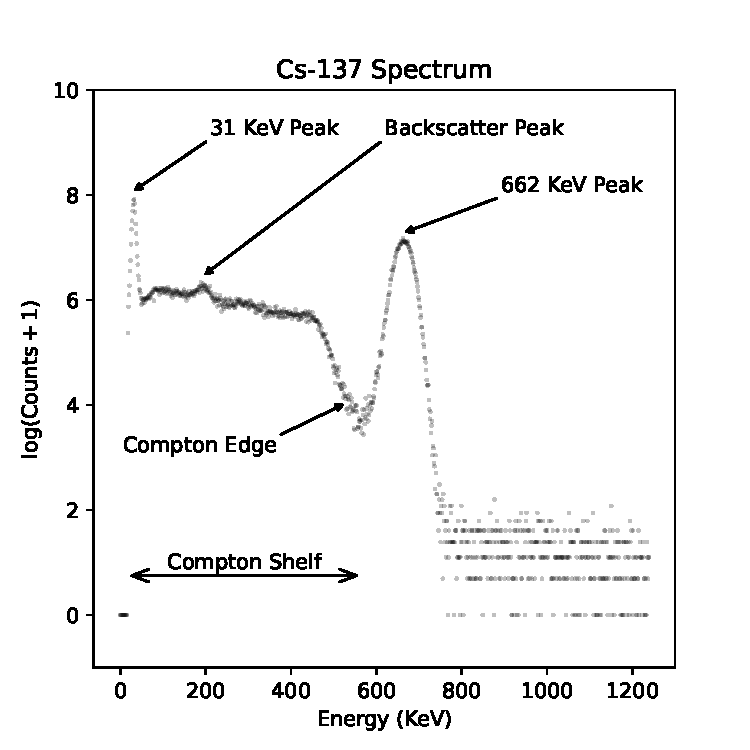
\includegraphics[width=0.5\textwidth]{experiment1/figures/cs137/spectrum.pdf}
    \caption{Spectrum of Cesium-137. Note the counts are in log scale, which creates the lines between 800 and 1200 KeV, where counts are low}
    \label{fig:cs137-spectrum}
\end{figure}

Figure \ref{fig:cs137-spectrum} shows a labeled spectrum collected, using our PMT setup, from a sample of Cesium-137. Figures \ref{fig:cs137-31} and \ref{fig:cs137-662} show close-up views of the two full energy peaks, along with appropriately fitted curves. 

\begin{figure}[h]
    \centering
    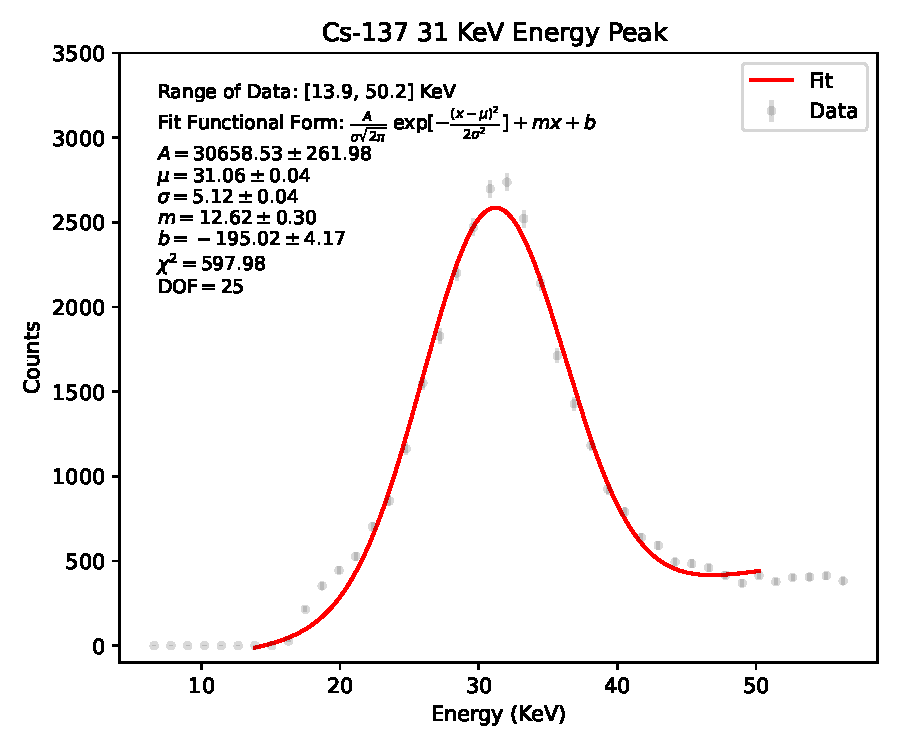
\includegraphics[width=0.5\textwidth]{experiment1/figures/cs137/peak-31.pdf}
    \caption{31 KeV Full Energy Peak of Cesium-137}
    \label{fig:cs137-31}
\end{figure}

We know from decay schemes that the first peak should be centered at 31 KeV. Our spectrum data in that region is relatively sparse due to the low gain we used, as shown by the low DOF count. Accordingly, our fitted curve fails to capture some of the data points near the peak and around the tails—hence the high $\chi^2$ score. The mean $\mu$ estimated by the fit is very close to 31 KeV, however the margin of error does not quite encompass it. This suggests some bias inherent in our setup. 

\begin{figure}[h]
    \centering
    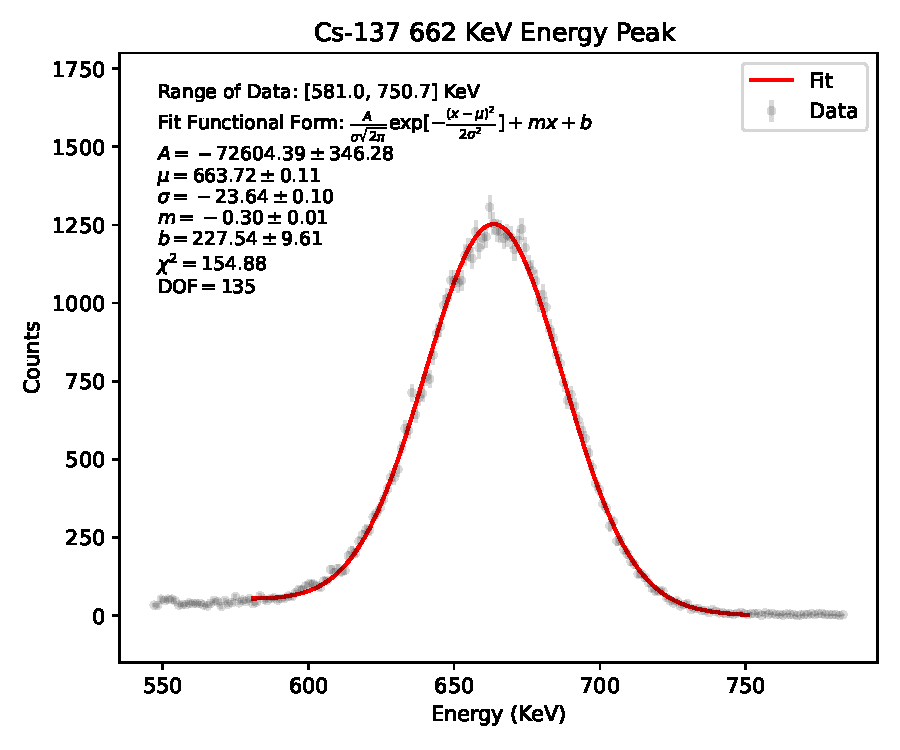
\includegraphics[width=0.5\textwidth]{experiment1/figures/cs137/peak-662.pdf}
    \caption{662 KeV Full Energy Peak of Cesium-137}
    \label{fig:cs137-662}
\end{figure}

We also know that the second peak should be centered at 662 KeV. At this energy, our data is relatively rich, with a high DOF, and the curve we fit nicely captures the visual distribution of the data with small $\chi^2$. Again, our estimated $\mu$ is close, but its margin of error does not capture the expected mean of 662 KeV. This is likely the same underlying bias that we observed when fitting the 31 KeV peak. 

\subsection{Sodium-22 Spectrum}

\begin{figure}[h]
    \centering
    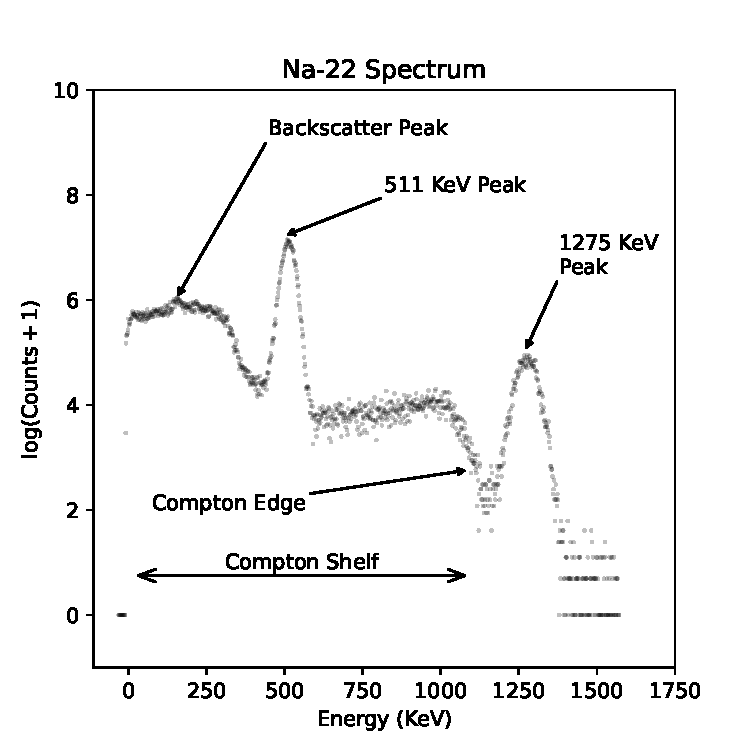
\includegraphics[width=0.5\textwidth]{experiment1/figures/na22/spectrum.pdf}
    \caption{Spectrum of Sodium-22. Note the counts in log scale. }
    \label{fig:na22-spectrum}
\end{figure}

Moving on to Sodium-22, the spectrum collected by the PMT is shown in Figure \ref{fig:na22-spectrum} and the two fitted full energy peaks in Figures \ref{fig:na22-511} and \ref{fig:na22-1275}. 

\begin{figure}[h]
    \centering
    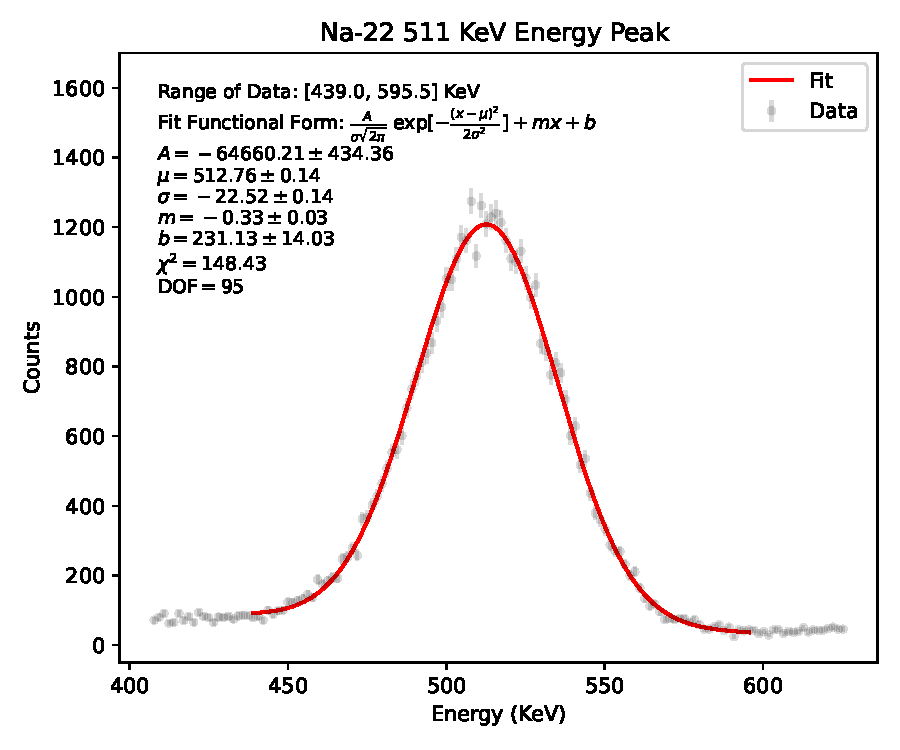
\includegraphics[width=0.5\textwidth]{experiment1/figures/na22/peak-511.pdf}
    \caption{511 KeV Full Energy Peak of Sodium-22}
    \label{fig:na22-511}
\end{figure}

The first peak should fall around 511 KeV. Here, we observe decently rich data with good DOF, and our fit is close, with a good $\chi^2$ score. As with our results for Cesium-137, we observe here that our mean is narrowly biased away from the expected value, and its margin of error is not large enough to explain this. 

\begin{figure}[h]
    \centering
    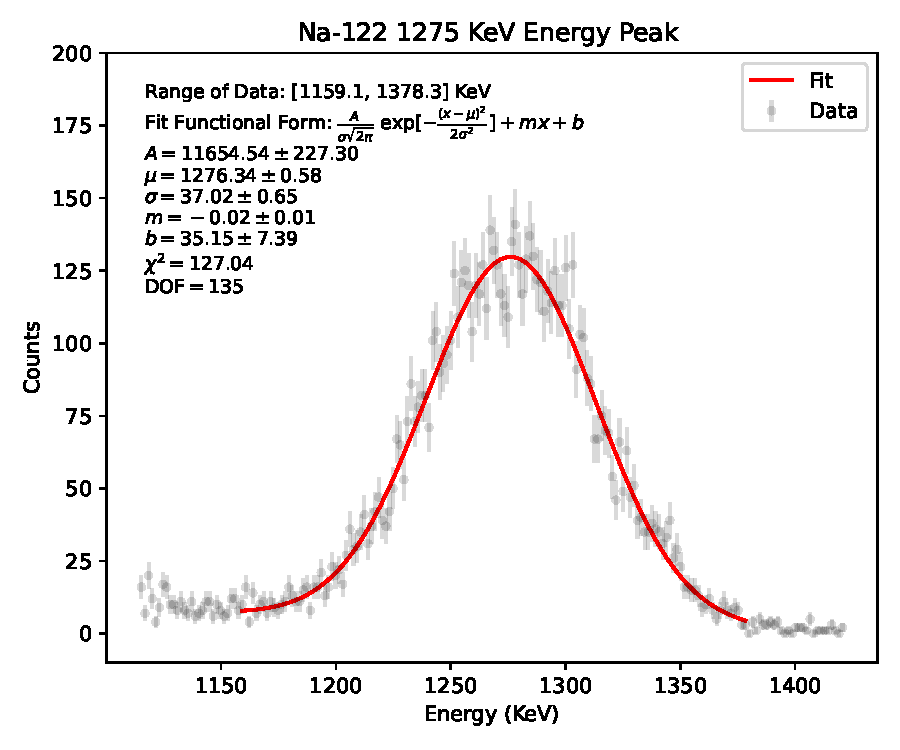
\includegraphics[width=0.5\textwidth]{experiment1/figures/na22/peak-1275.pdf}
    \caption{1275 KeV Full Energy Peak of Sodium-22}
    \label{fig:na22-1275}
\end{figure}

The second peak should fall around 1275 KeV. Here, the data is rich, albeit uncertain, with high DOF. The fit continues to be good with low $\chi^2$, and matches well the shape of the data. The bias issue we observe continues to manifest itself. 


\subsection{Barium-133 Spectrum}

\begin{figure}[h]
    \centering
    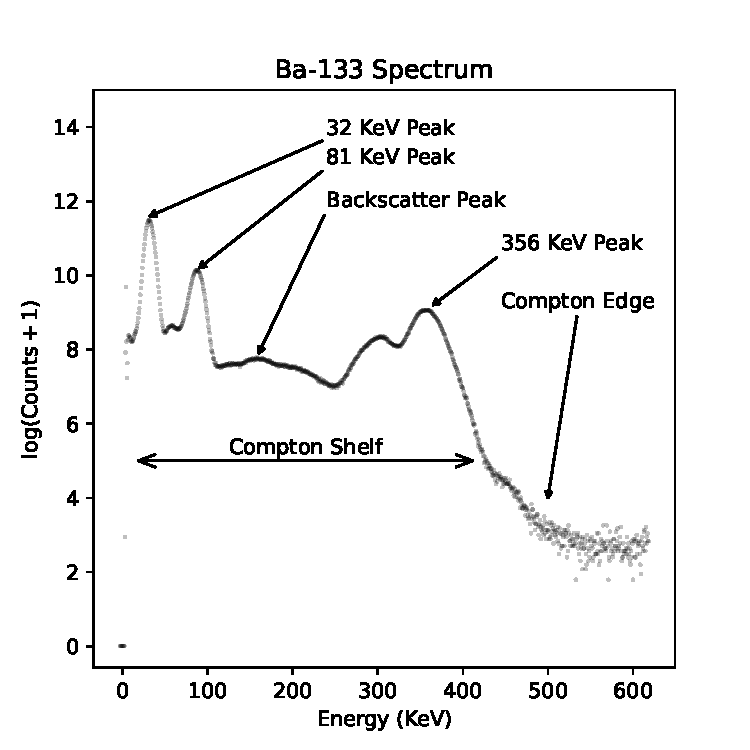
\includegraphics[width=0.5\textwidth]{experiment1/figures/ba133/spectrum.pdf}
    \caption{Spectrum of Barium-133. Note the counts in log scale.}
    \label{fig:ba133-spectrum}
\end{figure}

Finally, we consider Barium-133. Its PMT-collected spectrum is shown labeled in Figure \ref{fig:ba133-spectrum} and three full energy peaks in Figures \ref{fig:ba133-32}, \ref{fig:ba133-81}, and \ref{fig:ba133-356}. 

\begin{figure}[h]
    \centering
    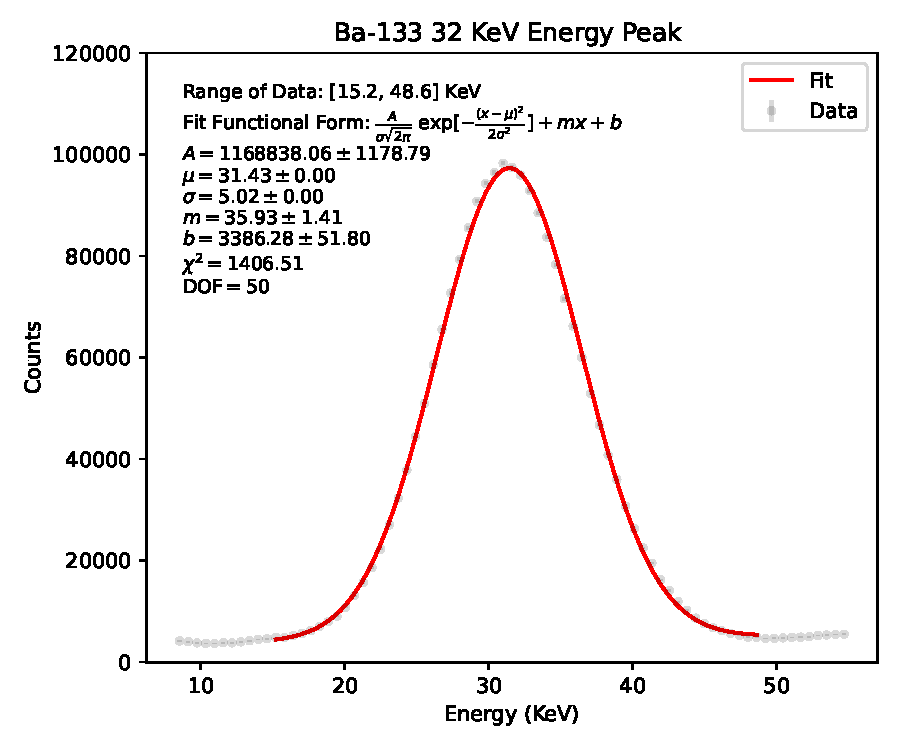
\includegraphics[width=0.5\textwidth]{experiment1/figures/ba133/peak-32.pdf}
    \caption{32 KeV Full Energy Peak of Barium-133}
    \label{fig:ba133-32}
\end{figure}

Similarly to the 31 KeV peak of Cesium-137, we observe sparse data for the 32 KeV peak of Barium-133. The DOF is low, however the fit is visually very good and the $\chi^2$ is low compared to the scale of the data. Again, we observe a bias due to a slightly deviating mean and low margins of error. 

\begin{figure}[h]
    \centering
    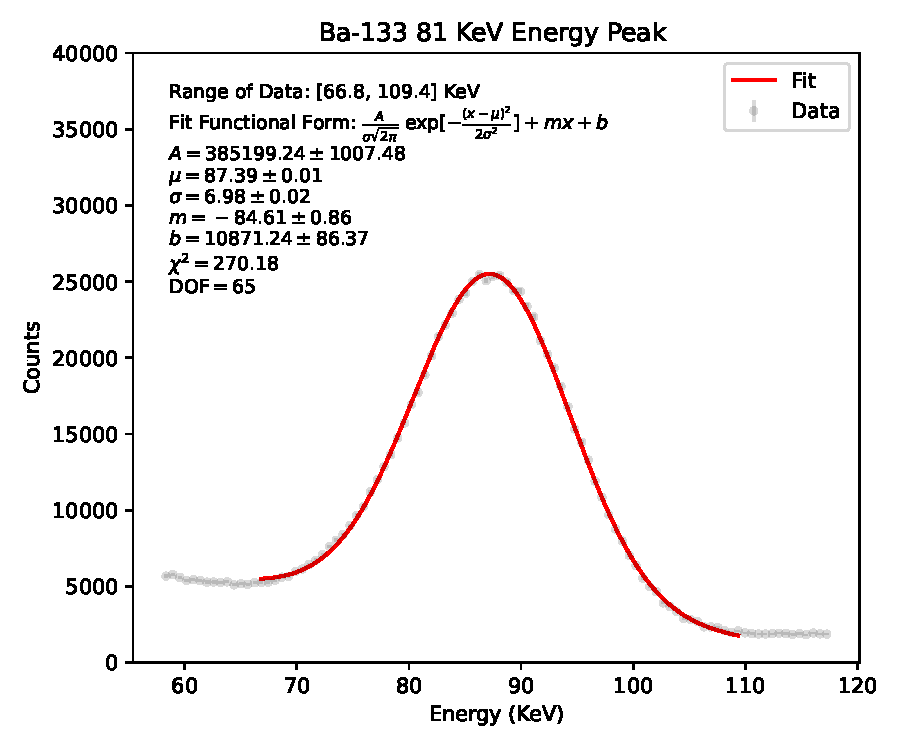
\includegraphics[width=0.5\textwidth]{experiment1/figures/ba133/peak-81.pdf}
    \caption{81 KeV Full Energy Peak of Barium-133}
    \label{fig:ba133-81}
\end{figure}

The 81 KeV peak continues the same trend, with good visual fit, low $\chi^2$, and a bias. This time, the bias is higher than we have previously observed, and accompanied by small margins of error. It is unclear why this energy peak is so much more biased than the others. Finding spectra with peaks around this magnitude may prove insightful. 

\begin{figure}[h]
    \centering
    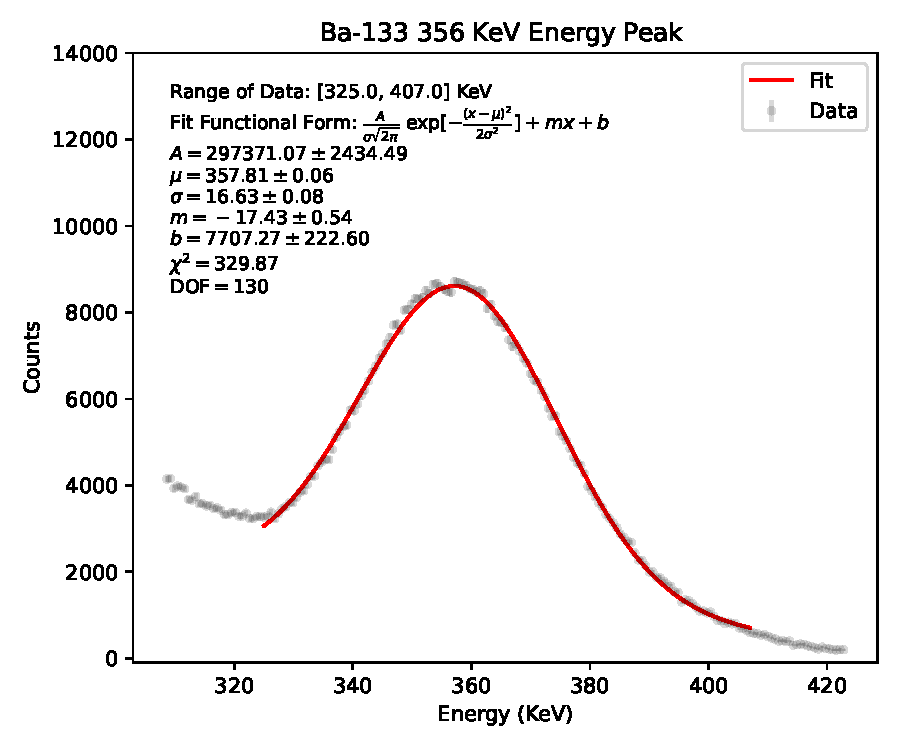
\includegraphics[width=0.5\textwidth]{experiment1/figures/ba133/peak-356.pdf}
    \caption{356 KeV Full Energy Peak of Barium-133}
    \label{fig:ba133-356}
\end{figure}

Finally, the 356 KeV peak returns to the original trend of good fit, low $\chi^2$, and a small bias unaccounted for by the margin of error. 

\subsection{Discussion of Observed Bias}

For all the energy peaks above, we observed a small bias in our fitted estimates of the mean. The low margins of error suggest that this is not a random bias, but rather a defect in our setup. One conjecture is that the bias from out of inaccurate calibration of the energy scale. This may explain why the bias for the 81 KeV peak of Barium-133 was unusually high—the energy was extrapolated from the calibration points around 32 and 356 KeV. 

\subsection{Extracting Linear Attenuation Coefficients of Aluminum}

The spectra we can collect with our PMT setups can be used to determine linear attentuation coefficients, often denoted $\lambda$, which describe an absorbent material's radiation shielding ability. Here, we will measure $\lambda$s for aluminum and determine how it performs absorbing different radiation of various energies. 

Our setup will remain mostly the same, though we now use aluminum blocks of various thicknesses as absorbers. Recall that when we measured the spectra, no absorbers were used. 

From theory, $\lambda$ is related to $R$, the rate at which photons pass through the absorber, and $x$, the thickness of the absorber, by: 
\[R = R_0 e^{-\lambda x}\]
$R$ is given by:
\[R = \frac{N}{T}\]
where $N$ is the number of photons from a radiation source that pass through the absorber in time $T$. 

Given a radiation source that emits radiation at known energies, we use the USX software to collect a spectrum. The spectrum is basically a histogram binned by photon energy. So, the photon counts can be found by checking the bins corresponding to the energies of interest. USX compiles two counts, $G$ is the gross count and $B$ is the background count. Since we wish to exclude background radiation, we use $N = G - B$. Accordingly, the error:
\[\delta N = \sqrt{\delta G^2 + \delta B^2} = \sqrt{\sqrt{G}^2 + \sqrt{B}^2} = \sqrt{G + B}\]
The error of $R$ is then:
\[\delta R = R * (\frac{\delta N}{N} + \frac{\delta T}{T})\]
where $\delta T$ is taken to be $1$ second. 

With this in mind, we measure $N$ and $T$ for various absorbers and various radiation energies. Then, we fit $R = R_0 e^{-\lambda x}$ curves and extract the $\lambda$s as estimates of the linear attenuation coefficients. 

\begin{figure}[h]
    \centering
    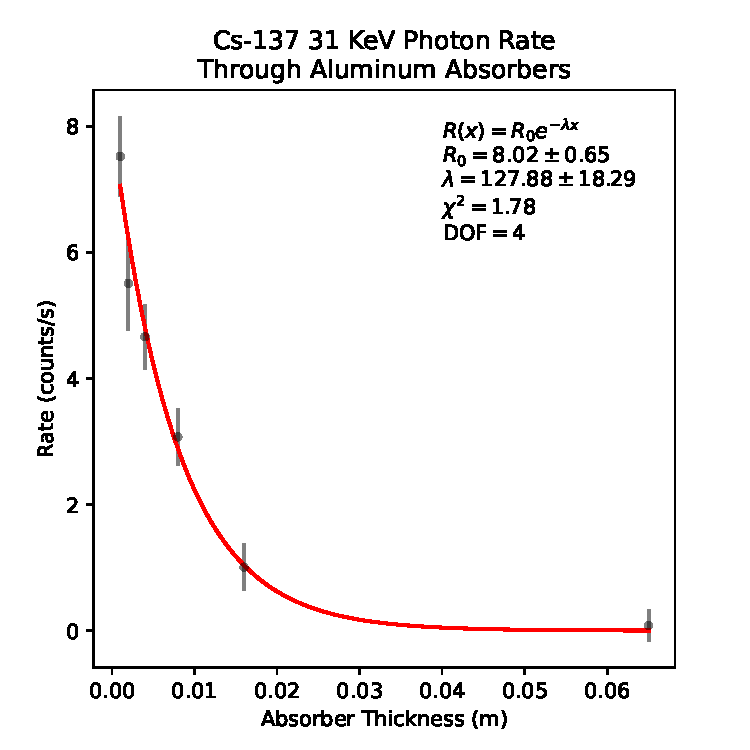
\includegraphics[width=0.5\textwidth]{experiment1/figures/cs137/rates-31.pdf}
    \caption{Photon Rate Curve at 31 KeV Gammas from Cesium-137}
    \label{fig:rates31}
\end{figure}

\begin{figure}[h]
    \centering
    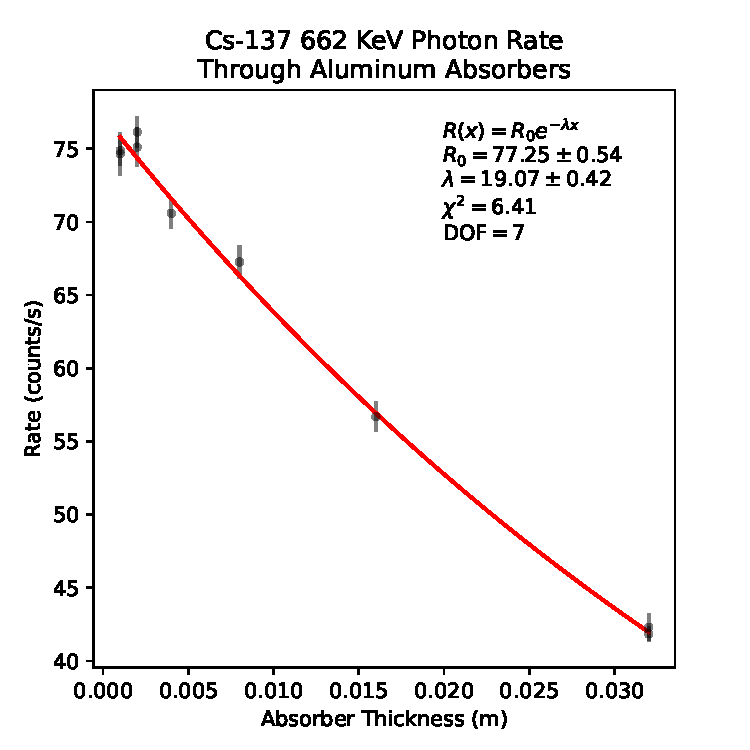
\includegraphics[width=0.5\textwidth]{experiment1/figures/cs137/rates-662.pdf}
    \caption{Photon Rate Curve at 662 KeV Gammas from Cesium-137}
    \label{fig:rates662}
\end{figure}

\begin{figure}[h]
    \centering
    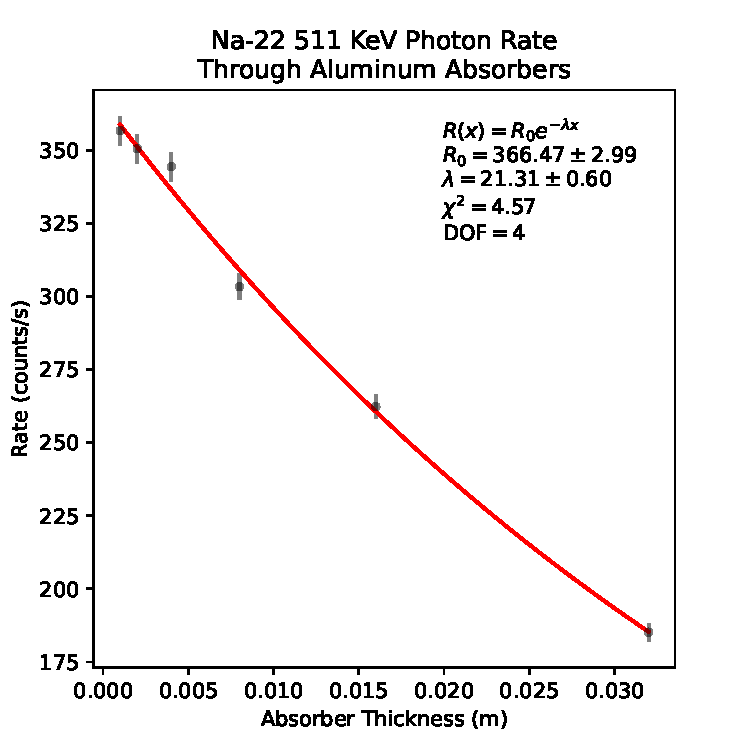
\includegraphics[width=0.5\textwidth]{experiment1/figures/na22/rates-511.pdf}
    \caption{Photon Rate Curve at 511 KeV Gammas from Sodium-22}
    \label{fig:rates511}
\end{figure}

\begin{figure}[h]
    \centering
    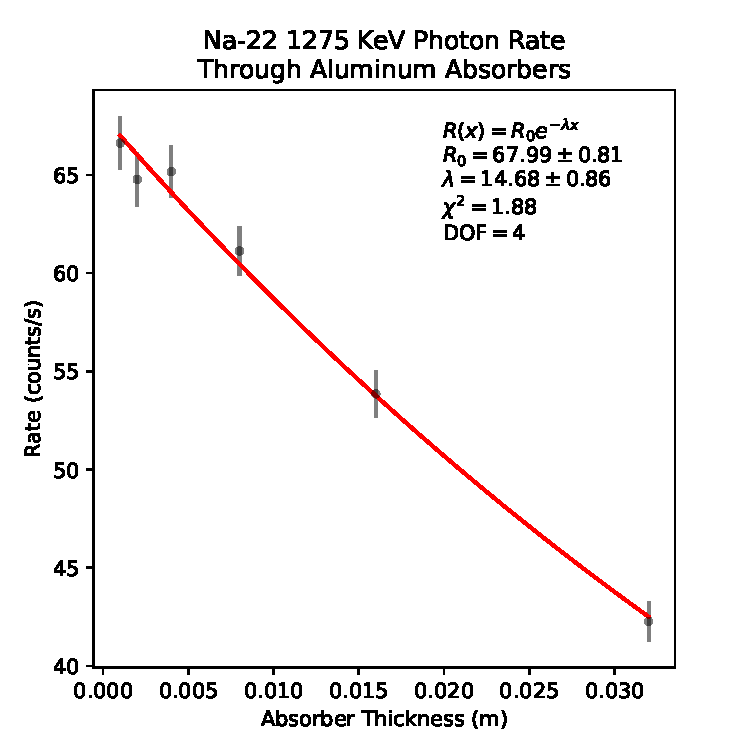
\includegraphics[width=0.5\textwidth]{experiment1/figures/na22/rates-1275.pdf}
    \caption{Photon Rate Curve at 1275 KeV Gammas from Sodium-22}
    \label{fig:rates1275}
\end{figure}

\begin{figure}[h]
    \centering
    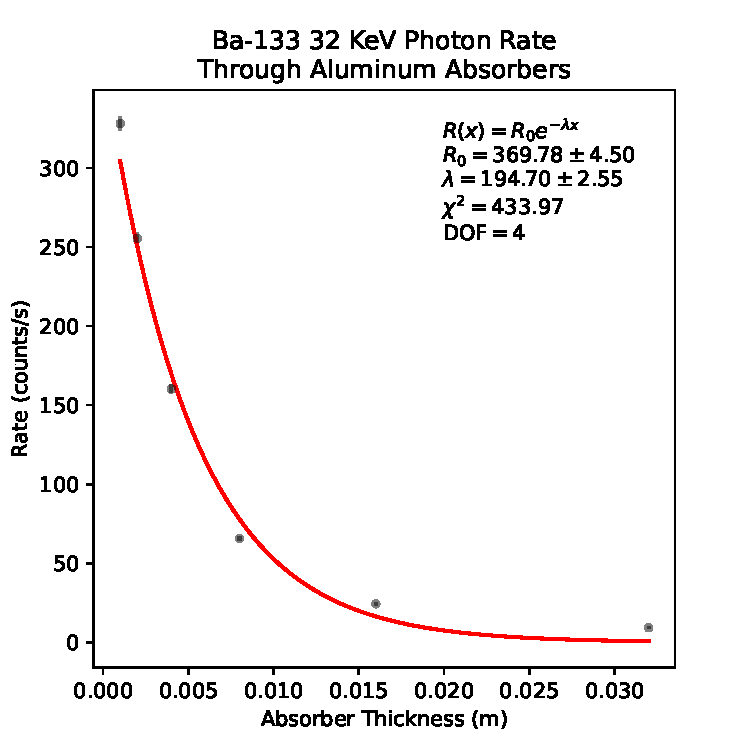
\includegraphics[width=0.5\textwidth]{experiment1/figures/ba133/rates-32.pdf}
    \caption{Photon Rate Curve at 32 KeV Gammas from Barium-133}
    \label{fig:rates32}
\end{figure}

\begin{figure}[h]
    \centering
    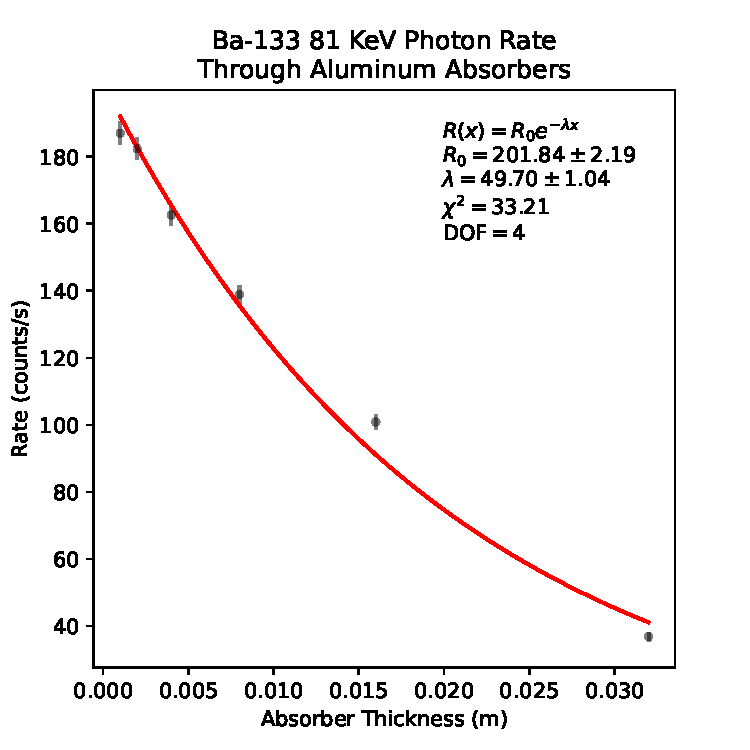
\includegraphics[width=0.5\textwidth]{experiment1/figures/ba133/rates-81.pdf}
    \caption{Photon Rate Curve at 81 KeV Gammas from Barium-133}
    \label{fig:rates81}
\end{figure}

\begin{figure}[h]
    \centering
    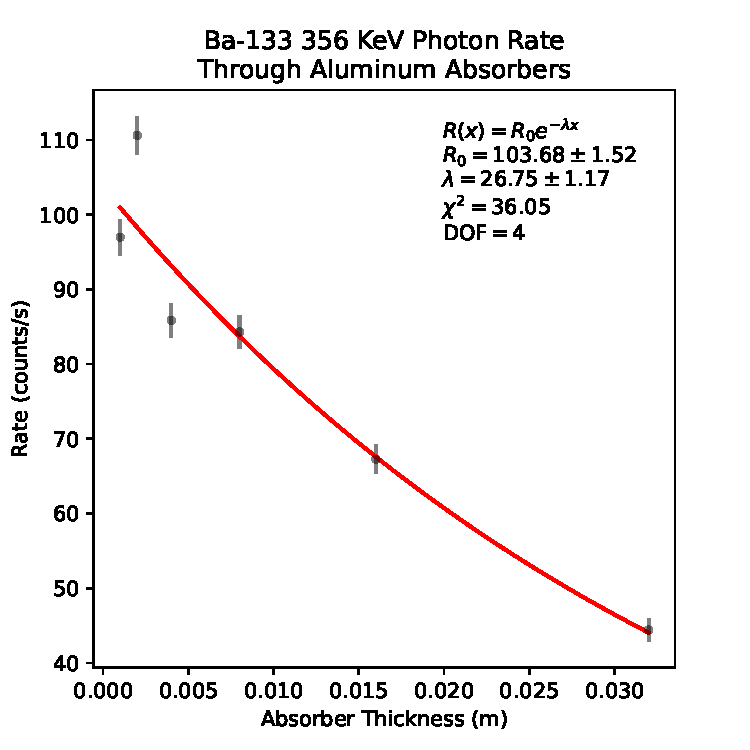
\includegraphics[width=0.5\textwidth]{experiment1/figures/ba133/rates-356.pdf}
    \caption{Photon Rate Curve at 356 KeV Gammas from Barium-133}
    \label{fig:rates356}
\end{figure}

In general, most of our the curves we regress exhibit small $\chi^2$ values, indicating good fit to the data. This supports the theoretical result that absorber thickness is related to photon rate as an inverse exponential. However, the data itself is sparse and has low DOF. In some of the plots, such as \ref{fig:rates356} it exhibits significant residual effects around the fitted curve. In part, this is due to the sparsity of the data. But systematic issues with our setup are also likely present. Namely, many of the thinner aluminum absorbers we used were bent, thus introducing error both within our thickness measurements and the aluminum's absorbing effect. 

\section{Conclusions}\label{sec:conclusion}

\begin{table}[h]
\centering
\begin{tabular}{|c | c c c c c c c |}
    \hline
    Energy (KeV) & 31 & 32 & 81 & 356 & 511 & 662 & 1275 \\
    \hline
    Fitted $\lambda$ & 127.9 & 194.7 & 49.7 & 26.8 & 21.3 & 19.1 & 14.7 \\
    Expected $\lambda$ & 279.2 & 256.7 & 54.1 & 26.7 & 22.6 & 20.2 & 14.7 \\
    \hline
\end{tabular}
\caption{Fitted and expected linear attentuation coefficients for various energy levels.}
\label{table:1}
\end{table}

From the fitted curves, we extract the values of $\lambda$ and compile them in Table \ref{table:1}. We also include expected values extrapolated from a s seen in Table \ref{table:1}, some of the fitted $\lambda$s are close to the expected values, but exhibit bias and margins of error that are too small. Other $\lambda$s stray far from the expectation. In general, our estimates are worse for low energy radiation, which may be attributable to poor spectrum data in those areas. 

\end{document}